\documentclass[12pt]{article}

% Packages
\usepackage[utf8]{inputenc}
\usepackage{amsmath}
\usepackage{amsfonts}
\usepackage{amssymb}
\usepackage{graphicx}
\usepackage{hyperref}
\usepackage{tikz}
\usepackage{fancyvrb}
\usepackage{multicol}
\usepackage{array}
\usepackage{amsmath}
\usepackage{tabularx}
\usepackage{tcolorbox}
\usepackage{float}

\usetikzlibrary{arrows.meta}
\hypersetup{
    colorlinks=true,
    linkcolor=black,
    citecolor=black,
}



% Document
\begin{document}

\title{Comparison in Concurrency Models in different programming languages}
\author{
    Christofer Washington Berruz Chungata \\ 
    Karan Jain \\ 
    Amey Makarand Dhongade \\ 
    \\
    San Jos\'{e} State University \\ 
    CS 252 - Final Project
}
\date{May 12, 2025}

\maketitle

\begin{abstract}
This project is very abstract
\end{abstract}

\section{Introduction\label{sec:introduction}}
This is my introduction

Concurrency in modern software systems needs abstractions that simplify reasoning and fully exploit distributed architectures as discussed in \cite{10.1145/357980.358021} . The Actor Model provides an abstraction by encapsulating state with independent actors that communicate only through asynchronous messaging. Each actor processes one message at a time from its mailbox, preventing data races and deadlocks. Strict encapsulation ensures that only the actor itself can read or update its internal state, thus not  needing locks. By decoupling senders and receivers, asynchronous messaging removes head-of-line blocking and allows flexible scheduling. Optimized mailbox implementations—ranging from lock-free, unbounded queues in Scalaz to bounded, configurable mailboxes in Akka tune enqueue and dequeue performance under varying workloads. Work-stealing dispatchers, such as those provided by Grand Central Dispatch or the fork-join pool, adapt automatically and balance load without manual thread management. This survey examines how mailbox structures, dispatcher strategies, and actor hierarchies interact to optimize scalability, fault tolerance, and programmability in actor-based systems.

\section{Background\label{sec:background}}
Background.

\section{Shared-Memory Model\label{sec:shared_memory}}
A shared-memory concurrency model is any model in which units of computation,
processes or threads, communicate with each other using shared memory.
Communication is done by reading and writing to a shared object. Refer to
\autoref{fig:shared_memory} for a visual representation of the shared-memory model.

% shared memory figure
\begin{figure}[!htp]
    \centering
    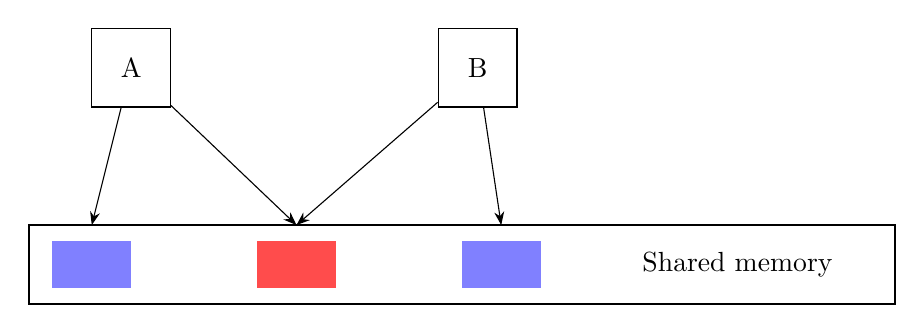
\begin{tikzpicture}[node distance=1cm and 1.5cm, >=Stealth]

        % Shared memory bar
        \draw[thick] (0,0) rectangle (11,1);
        \node at (9,0.5) {Shared memory};
      
        % Memory blocks
        \fill[blue!50] (0.3,0.2) rectangle (1.3,0.8);
        \fill[red!70] (2.9,0.2) rectangle (3.9,0.8);
        \fill[blue!50] (5.5,0.2) rectangle (6.5,0.8);
      
        % Processes A and B
        \node[draw, minimum width=1cm, minimum height=1cm] (A) at (1.3,3) {A};
        \node[draw, minimum width=1cm, minimum height=1cm] (B) at (5.7,3) {B};
      
        % Arrows from processes to memory blocks
        \draw[->] (A) -- (0.8,1);
        \draw[->] (A) -- (3.4,1);
        \draw[->] (B) -- (3.4,1);
        \draw[->] (B) -- (6.0,1);
      
      \end{tikzpicture}
      \caption{
        Shared-memory concurrency model. 
        Processes A and B communicate by reading and writing to shared memory blocks.
      }
      \label{fig:shared_memory}
\end{figure}

Note that the definition of \textit{memory} can be loosened depending on the application.
For example,~\cite{mitConcurrency} illustrates the following scenarios
where shared-memory concurrency models are applicable:

\begin{enumerate}
    \item A, B can be two processes communicating using the same process memory.
    \item A, B can be two programs communicating using the same filesystem.
    \item \label{itm:shared_object} A, B can be two running threads of some computer program
        communicating using the same object.
\end{enumerate}

When discussing limitations, advantages, or disadvantages of shared-memory concurrency models,
we will illustrate them using the scenario described in \autoref{itm:shared_object}.

\subsection{The Canonical Example}

The paper in~\cite{jaffe2011impactOfMemoryModels} describes a well-known canonical example.
Assume that we need to update a variable $x$ and increment it by $2$.
Assuming $x$ is already initialized, we can create two threads, $T_1$ and $T_2$, that will
increment $x$ by $1$ each. The code for both threads is shown in \autoref{fig:lost_update}.

Note that if both threads read the value of $x$ at the same time,
the final value of $x$ will be $1$. In fact, there's no guaranteed execution
order between $T_1$, and $T_2$ as the instructions can be interleaved
in any order. The interleaving problem is made more complex
due to the fact that most modern hardware can re-order instructions
\cite{huang2016debuggingConcurrentPrograms}. Furthermore, interleaving
makes it difficult to reproduce bugs, creating \textit{Heisenbugs}~\cite{rookout2021heisenbug,
gray1986whyComputersStop}.

%figure for the canonical example
\begin{figure}[!htp]
    \centering
    \begin{tabular}{|p{0.3\linewidth}|p{0.3\linewidth}|}
        \hline
        \textbf{$T_1$} & \textbf{$T_2$} \\
        \hline
        \begin{Verbatim}[fontsize=\small]
    int loc = x;
    loc = loc + 1;
    x = loc;
        \end{Verbatim}
        &
        \begin{Verbatim}[fontsize=\small]
    int loc = x;
    loc = loc + 1;
    x = loc;
        \end{Verbatim}
        \\
        \hline
    \end{tabular}
    \caption{Canonical example for shared-memory models.}
    \label{fig:lost_update}
\end{figure}

\subsection{Synchronization Mechanisms}
Synchronization mechanisms aim to solve the problems caused by interleaving: race conditions.
As the name implies, synchronization mechanisms synchronize the execution of multiple threads.
These mechanism are used in the critical sections of a program.
The most common synchronization mechanisms include synchronization primitives,
and atomic instructions~\cite{leroy2021sharedMemorySlides}. Note that message passing is a synchronization
mechanism, but it is highly used in the Communicating Sequential Processes (CSP) model.

\begin{tcolorbox}[colback=blue!5!white, colframe=blue!75!black, title=Critical Section]
    Critical sections are a series of instructions in a program that cannot
    be interleaved among multiple threads to guarantee the correctness of the program.
\end{tcolorbox}

Synchronization primitives allow
only certain threads to access a shared object at a time.
Locks, mutexes, semaphores, barriers, conditional variables, and monitors
are examples of synchronization primitives.
These mechanism are briefly described in \autoref{tab:mutualExclusionPrimitives}.

\begin{table}[!htp]
    \caption{Comparison of mutual exclusion mechanisms}
    \label{tab:mutualExclusionPrimitives}
    \centering
    \begin{tabularx}{\textwidth}{|l|X|X|}
        \hline
        \textbf{Primitive} & \textbf{Description}\\
        \hline
        Locks & 
        Simples mechanism. Allows only one thread at a time to access a shared object.\\
        \hline
        Mutexes & 
        Similar to a lock, but it can used system wide to synchronize multiple processes.\\
        \hline
        Semaphores & 
        Generalization over a lock: allow $N$ entities to access the resource at a time\\
        \hline
        Barriers &
        Given $N$ threads, all threads block until $P$ threads reach a section.\\
        \hline
        Conditional variables &
        Allows threads to wait for a condition to be true. Enhancement
        over semaphores with wait and signal operations.\\
        \hline
        Monitors &
        High-level abstraction over locks and condition variables. It packages
        the shared object and the synchronization primitives together.\\
        \hline
    \end{tabularx}
\end{table}

The biggest problem with synchronization primitives is that they can
lead to deadlocks when used incorrectly. Note that
the responsibility of avoiding deadlocks falls directly on the developer.
A deadlock occurs when two or more threads are waiting
for each other to release a resource, blocking \textbf{forever}.
When a deadlock occurs, the \textit{progress} property
of the system is violated. All synchronization mechanisms aim
at guaranteeing some of these three properties:
mutual exclusion, progress, and bounded waiting~\cite{csf2025synchronizationPrimitives}.


Given that it is difficult to not only know which synchronization
primitives to used, but also how to use them correctly,
several well-known patterns exist to create
correct concurrent programs: signaling,
turnstiles, rendezvous, multiplexes, and lightswitches~\cite{csf2025synchronizationDesign}.

\subsection{Memory Consistency Models}
One subtle implication of shared-memory models is that instructions
from all threads must be organized in \textbf{some order}. The reason is straightforward:
they are all accessing the same memory. Given that memory is unique and shared (hardware resource),
multiple threads cannot access the same memory address at the same time. Note that
we make the distinction between instructions and lines of code. The instructions
can be arranged in any order, regardless of how the lines of code are written.

A memory consistency model defines the set of rules that dictate how
instruction can be ordered, or interleaved, in a concurrent
program~\cite{bornholt2016memoryModels,jaffe2011impactOfMemoryModels}.
In concrete, the ordering rules focus on how \textbf{load} and \textbf{store} instructions
can be reordered. A load instruction reads a value from memory,
while a store instruction writes a value to memory.

Sequential Consistency (SC) is the strongest
and most intuitive model ~\cite{lamport1979multiprocessor}.
To guarantee SC, the system must ensure two properties~\cite{jaffe2011impactOfMemoryModels}:
\begin{enumerate}
    \item All threads must see the global order of memory operations.
    \item the operations of a particular property must appear to execute
    in program order.
\end{enumerate}

Although SC is extremely popular due to its high-level of abstraction,
its strictness is detrimental to performance because it limits
optimizations around memory access including caching,
dynamic scheduling, and pipelining. As a result, several relaxed
memory consistency models have been proposed:
Total Store Order (TSO), Partial Store Order (PSO),
and Weak Ordering (WO)~\cite{jaffe2011impactOfMemoryModels}.
Note that most modern hardware architectures implement a relaxed
memory consistency model, with Intel's x86 architecture implementing TSO~\cite{cox2021hardwareMemoryModels}.

Recall that the canonical example in \autoref{fig:lost_update}
demonstrates the interleaving problem. Given that memory
consistency models define how instructions can be rearranged,
they can either exacerbate or mitigate concurrency bugs
caused by undesirable interleaving.

The authors in~\cite{jaffe2011impactOfMemoryModels} show that
as the number of threads increases, the probability
of a concurrency bug manifesting is the same across strict and relaxed
memory consistency models. However, when two threads are used,
weak memory models do increase such probability. The experiment setup
is pretty straightforward: given a critical section for a program
similar to \autoref{fig:lost_update}, and a
memory consistency model, the authors are able to possibly
expand the critical window by reordering instructions.
Then, they are able to measure the probability of a concurrency
by taking into factoring in the size of the critical window
in their probabilistic model.
Note that these findings are not experimental, but rather
mathematically proven.

\section{Actor Model\label{sec:actor}}
An actor model is a type of concurrency model where the individual workers are the actors. An actor is an independent worker which has its own private state. Actors communicate by sending and receiving asynchronous messages. Each actor processes exactly one message at a time.

\subsection{Understanding the Actor Model Design}
The authors in~\cite{8316391} discuss the actor model design by first introducing the actor context. The actor context is the environment where the actors live. It creates actors, tracks them, routes messages to the right actor's mailbox.  The actor is the main unit of work done, in which each actor has a private state, has a mailbox attached, can send messages to other actors and process messages. The mailbox is where the incoming messages for the actor are stored. Processing is not done immediately, but whenever ready, the actor picks up a message from its mailbox and processes it. 
The actor model is illustrated in Figure~\ref{fig:actor}. 
\begin{figure}[H]
    \centering
    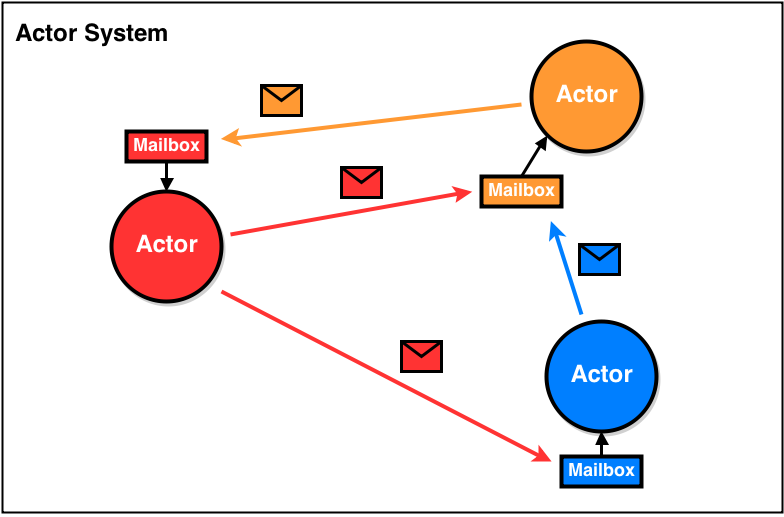
\includegraphics[width=0.7\textwidth]{actor.png}
    \caption{Actors communicating with other actors.}
    \label{fig:actor}
\end{figure}
\subsection{The Actor Model Principle}
The authors in~\cite{8316391} have also discussed regarding certain principles implemented in the actor model. Please refer to Table~\ref{tab:actor_model} for understanding the principles outlined in the actor model.

\begin{table}[H]
    \centering
    \caption{Basic Components of the Actor Model}
    \label{tab:actor_model}
    \begin{tabularx}{\textwidth}{|l|X|}
        \hline
        \textbf{Principle} & \textbf{Description} \\
        \hline
        Encapsulation & Each actor has a private internal state, and no actor can view it \\
        \hline
        Internal State & Each actor has its own memory and updates it. \\
        \hline
        Messaging & Actors communicate by sending and receiving \\
        \hline
        Indeterminacy & Messages may arrive in any order \\
        \hline
        
    \end{tabularx}
\end{table}

\subsection{Data Races and Deadlocks}
A data race occurs when when two or more threads access the same shared memory at the same time, which can corrupt the data. A deadlock occurs when two or more threads are waiting for each other to release a lock and so the system freezes. 

Data races don't occur in the actor model because there is no shared memory between actors, as each actor has its own private state, wherein no other actor can directly read or write that state and every communication happens through messages only. 

Deadlocks don't occur in the actor model as there is asynchronous messaging without any locks. Actors send a message and move on without waiting or blocking. In this no actor is waiting or holding a lock to release a resource.

\subsection{Optimization using Batch Actors}
The authors in~\cite{10820772} introduced batch actors to tackle the problem where hundreds of thousands of small tasks all try to synchronize through one actor, which can lead to a communication bottleneck.

Instead of using one main actor executing thousands of tasks, several tasks are grouped under batch actors, and batch actors message the main job actor, which leads to a reduce in contention. 

The experiments had shown that the models were 4x faster than the actor model without batching and resulted in less communication bottlenecks and better scaling.

\subsection{Benchmarks conducted}
The authors in~\cite{8892329} conducted various experiments using different libraries implementing the actor model. These were the findings:

\begin{table}[!htp]
    \centering
    \caption{Benchmarks and key findings from actor system implementations.}
    \label{tab:benchmarks_conducted}
    \begin{tabularx}{\textwidth}{|>{\raggedright\arraybackslash}X|>{\raggedright\arraybackslash}X|>{\raggedright\arraybackslash}X|}
        \hline
        \textbf{Benchmark} & \textbf{What it Measured} & \textbf{Main Finding} \\
        \hline
        Enqueuing Benchmark & Time taken to push messages into an actor's mailbox. & Scalaz achieved the fastest enqueuing time compared to Akka and Lift. \\
        \hline
        Max Throughput Benchmark & Number of messages processed per second. & Scalaz had the highest throughput performance. \\
        \hline
        Ping Latency Benchmark & Time for a message to travel from one actor to another and back. & Scalaz demonstrated the lowest ping latency. \\
        \hline
        Big Benchmark (Many-to-Many) & Performance under massive actor communication between many actors. & Scalaz scaled better with many actors under stress. \\
        \hline
        Chameneos Benchmark & Handling complex meeting and communication scenarios among actors. & Scalaz outperformed Akka and Lift in this concurrency problem. \\
        \hline
    \end{tabularx}
\end{table}

For pure speed, Scalaz is best for lightweight, fast concurrent systems. But for building robust, distributed systems, Akka is better becauser it offers more built-in tools as well as a good actor lifecycle management and for building complex and fault tolerant systems









\section{Software Transaction Memory\label{sec:stm}}
As introduced earlier, STM is a concurrency control mechanism that allows multiple threads to access shared memory in a way that avoids the need for locks.This section will provide a survey of various STM implementations, the design choices - the problems it aims to solve, and its advantages and disadvantages.
\subsection{Haskell}
Haskell has a strong emphasis on immutability and pure functions. This makes it an ideal candidate for STM, as it allows for easier reasoning about concurrent programs.  Haskell is purely functional with a strong type system; most data is immutable, and the side-effects including I/O are tightly controlled by monads. 

\begin{longtable}{|p{0.2\textwidth}|p{0.3\textwidth}|p{0.4\textwidth}|}
    \caption{Design choices for Haskell STM} \label{tab:Haskell-STM Design Choices} \\
    \hline
    \textbf{Design Primitive} & \textbf{Associated Hazards} & \textbf{Reason for Use} \\
    \hline
    \endfirsthead
    \hline
    \textbf{Design Primitive} & \textbf{Associated Hazards} & \textbf{Reason for Use} \\
    \hline
    \endhead
    \hline
    \endfoot
    \hline
    \endlastfoot
    \codeify{TVar} & 
    Memory overhead from versioning; restricted mutation outside transactions &	
    Enables optimistic concurrency control while maintaining type safety. Prevents direct access to shared state outside transactions. \\
    \hline
    \codeify{retry} &
    Indefinite blocking if dependencies never change &
    Automatically restarts transactions only when relevant state changes, avoiding busy waiting. Enabled by dependency tracking via TVar versioning. \\
    \hline
    \codeify{orElse} &
    Increased contention if alternatives access overlapping TVars &	
    Allows composable transaction alternatives without manual coordination. Reduces need for nested exception handling. \\
    \hline
    \codeify{type-enforced STM/I/O separation} &
    Limits expressiveness (no I/O in transactions) &
    Ensures transactions remain rollback-safe. Leverages Haskell's purity to avoid irreversible side effects. \\
    \hline
    \codeify{optimistic concurrency (no locks)} &
    High retry rates under contention &	
    Avoids lock acquisition overhead in common cases. Aligns with Haskell's allocation-heavy workloads where conflicts are rare. \\
    \hline
    \codeify{per-thread transaction logs} &	
    Memory overhead scaling with thread count &	
    Enables lock-free progress guarantee: at least one thread always commits without global synchronization. \\
    \hline
    \codeify{global version clock} &
    Clock overflow risk (64-bit memory address space) &
    Provides a consistent view of shared state across threads. Avoids global synchronization for version updates. \\
    \hline
    \codeify{phase-fair reader/writer locks} &
    Priority inversion in contended writes &
    Ensures progress for both readers and writers. Critical for real-time systems using STM. \\
    \hline
    \codeify{eager conflict detection} &
    False positives in long transactions &
    Minimizes wasted work by aborting early. Complements optimistic approach by failing fast. \\
    \hline
    \codeify{block-structured heap} &
    Memory fragmentation from large objects &
    Enables efficient parallel GC. Allows STM metadata (TVar versions) to coexist with regular objects. \\
    \hline
    \codeify{cooperative multitasking} &
    STM deadlocks in allocation-free loops &
    Avoids OS thread overhead. Mitigated by -fomit-yields flag inserting yield points. \\
    \hline
    \codeify{blackhole-based thunk evaluation} &
    Duplicated computation in races &
    Prevents multiple threads evaluating same thunk. Uses CAS for thread-safe lazy evaluation. \\
    \hline
\end{longtable}
This environment mitigates many STM pitfalls like preventing I/O inside transactions (you must use retry or other STM primitives), so the “invisible I/O” problem is solved by the type system. The result is that Haskell STM can offer robust, composable concurrency abstractions (e.g. transactional queues TBQueue, TChan, etc.) with minimal unexpected interactions.


\subsection{Clojure}
Clojure’s entire identity/state model was built with STM in mind. Clojure’s data structures are immutable and persistent, and the only way to have coordinated shared state is via refs in a dosync block. Rich Hickey’s rationale emphasizes “immutable persistent data structures” plus “built-in concurrency support via STM and asynchronous agents” \cite{clojure.org}.



In practice though, many Clojure programs end up using simpler primitives like atoms or persistent queues, but the option of STM is always there and shapes how other features work. For instance, atoms (lock-free single-ref updates) only make sense because data is immutable, a design inspired by STM’s snapshot view\cite{news.ycombinator.com}. Even if Clojure refs aren’t used “99.9\% of the time”, the fact that the language and libraries expect STM means that concurrency is built on a solid foundation of the immutable design, which were designed for STM.

\subsection{Rust}
Rust is a systems programming language that emphasizes safety and performance. It has a strong type system and ownership model, which makes it an ideal candidate for STM. Rust's ownership model ensures that data is either mutable or immutable, which helps to prevent side effects in away that is similar to Haskell. Rust's type system also allows for easy reasoning about concurrent programs, as it enforces strict rules about data access and ownership.

These features are implemented through external liraries like stm and async-stm-rs. Former provides STM support for Rust, while the latter async programming support for Rust.
We also look at design choices of an expermimental STM implementation called TORTIS which stands for Try Once.
It uses a new method for STM called R2STM, which is a hybrid of optimistic and pessimistic concurrency control. It uses a combination of locks and transactions to provide a more efficient and scalable STM implementation. The design choices for TORTIS are as follow:\\


\subsection{Abandonement}

While STM is a powerful concurrency control mechanism, it is not without its challenges. Some prominent implementations have been abandoned due to various reasons, including performance issues, complexity, and lack of community support :
\begin{enumerate}
    \item \textbf{.NET:}  Microsoft (MS) had an adaptation of STM :  STM.NET, that was pulled by 2010. Joe Duffy (lead researcher for parallelism and concurrency at MS) and colleagues found less or no compelling workloads that needed STM. Duffy notes that their final discouraging verdict: many concurrency apps “enjoyed natural isolation,” and heavy sharing often meant “you were doing something wrong"\cite{infoq.com}.  In its place, .NET heavily promoted Task Parallel Library (TPL), PLINQ for data parallelism, async/await for async I/O, and concurrent collections as simpler models.
    \item \textbf{Python:}  Standard CPython(C-based Interpreter) still has a Global Interpreter Lock (GIL), so technically only one thread executes Python bytecode at a time, thereby limiting true parallelism. Efforts like an experimental STM-based PyPy which uses RPython (R-based Interpreter), attempted to remove the GIL by wrapping every Python bytecode in transactions. \cite{pypy.org}. This allowed multiple threads to run atomic blocks concurrently, rolling back on conflicts. The approach proved complex and was not adopted to mainstream ; instead multiprocessing, asyncio/event loops, and external libraries like Celery took over.
    \item \textbf{Akka:} Around the same time as .NET abandonment, Akka also abandoned its STM implementation.Akka used the Multiverse library and Clojure-style refs for advanced use cases
    \cite{doc.akka.io}. However, Akka is fundamentally about the actor model, where each actor has private state and interacts by message passing, unlike STM’s shared-memory transactions. Akka tech lead Roland Kuhn notes that STM was “considered a failed experiment” in their context and “never compatible with distributed computing”.
\end{enumerate}


% Bibliography
\bibliographystyle{plain}
\bibliography{references}

\end{document}